
\begin{figure}[ht]
  \centering

  \begin{subfigure}[b]{0.45\textwidth}
    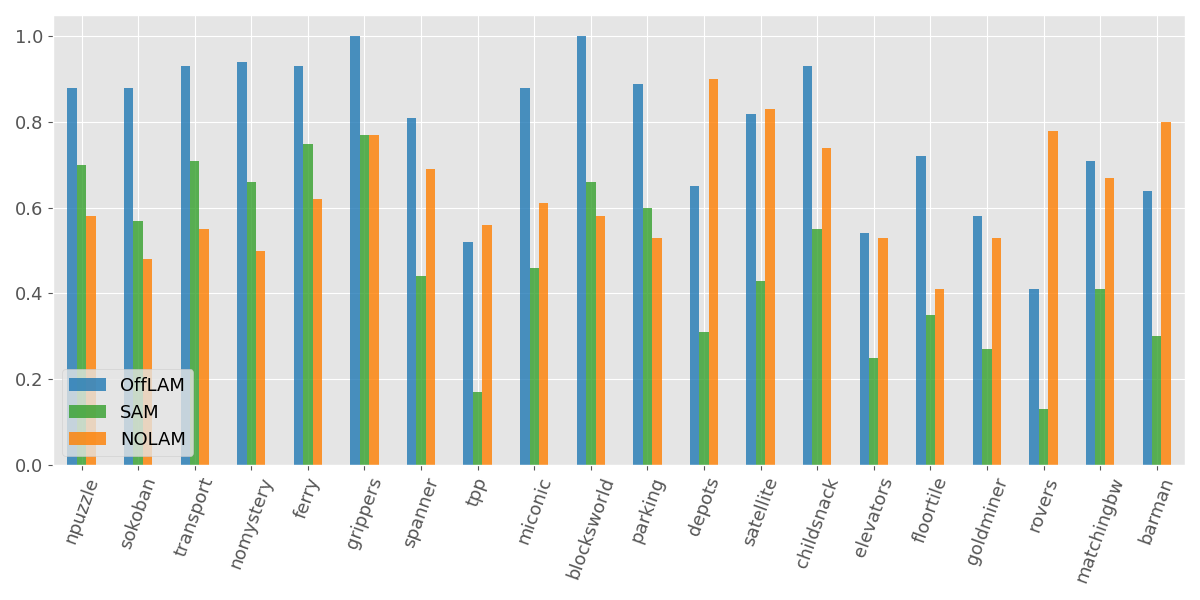
\includegraphics[width=\textwidth]{figures/2_traces/syn_precision.png}
    \caption{Syntactic precision}
  \end{subfigure}
  \hfill
  \begin{subfigure}[b]{0.45\textwidth}
    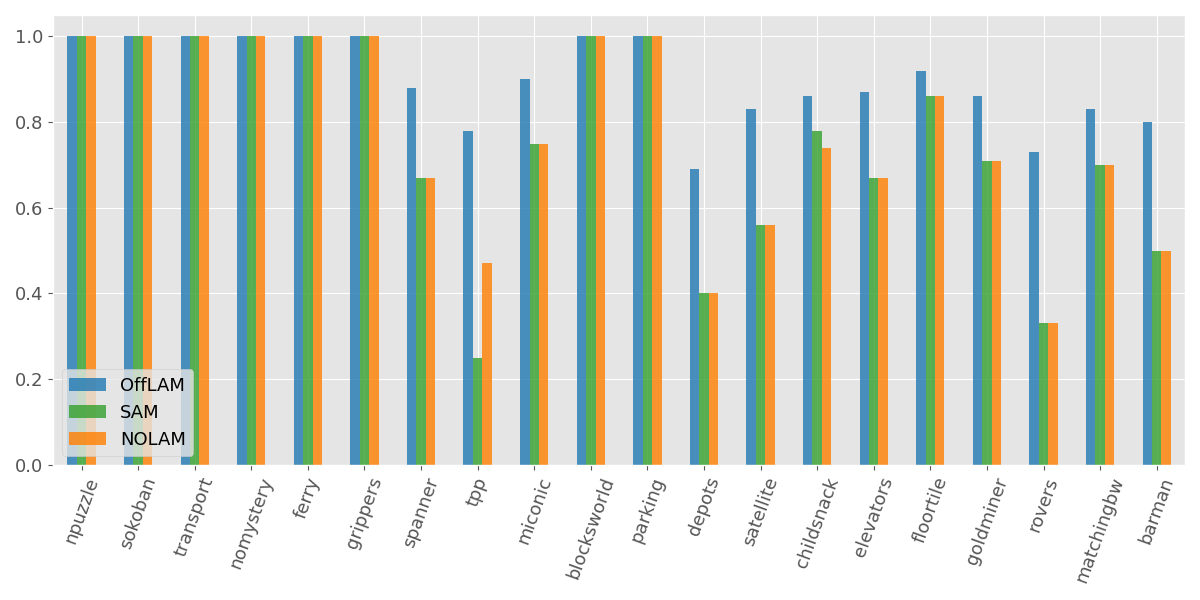
\includegraphics[width=\textwidth]{figures/2_traces/syn_recall.png}
    \caption{Syntactic recall}
  \end{subfigure}

  \vspace{1em}

  \begin{subfigure}[b]{0.45\textwidth}
    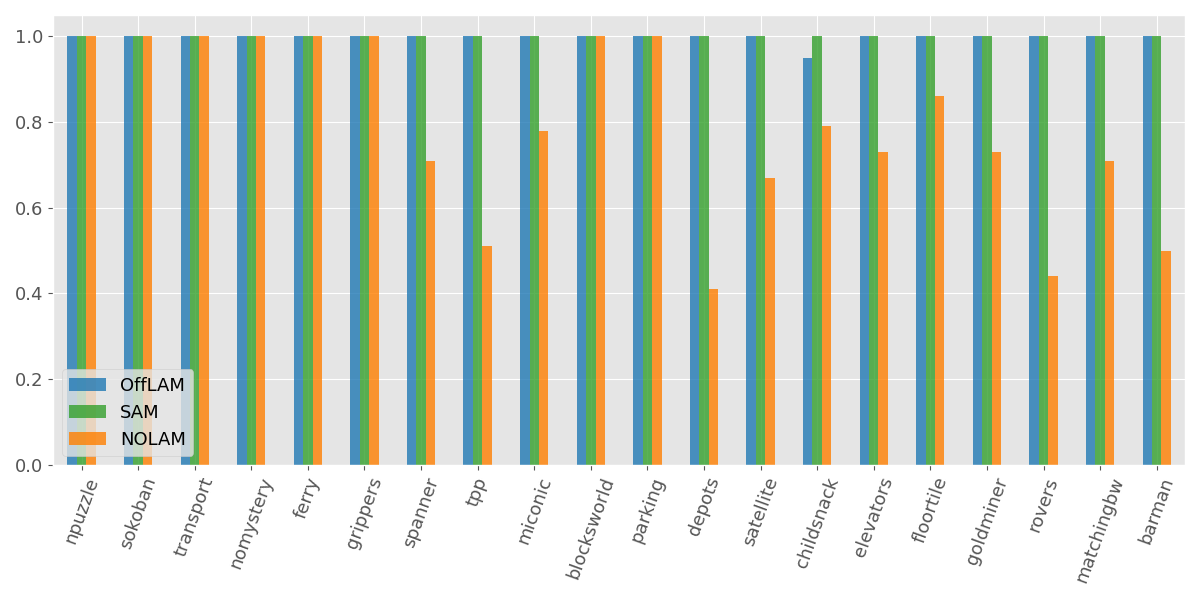
\includegraphics[width=\textwidth]{figures/2_traces/app_precision.png}
    \caption{Applicability precision}
  \end{subfigure}
  \hfill
  \begin{subfigure}[b]{0.45\textwidth}
    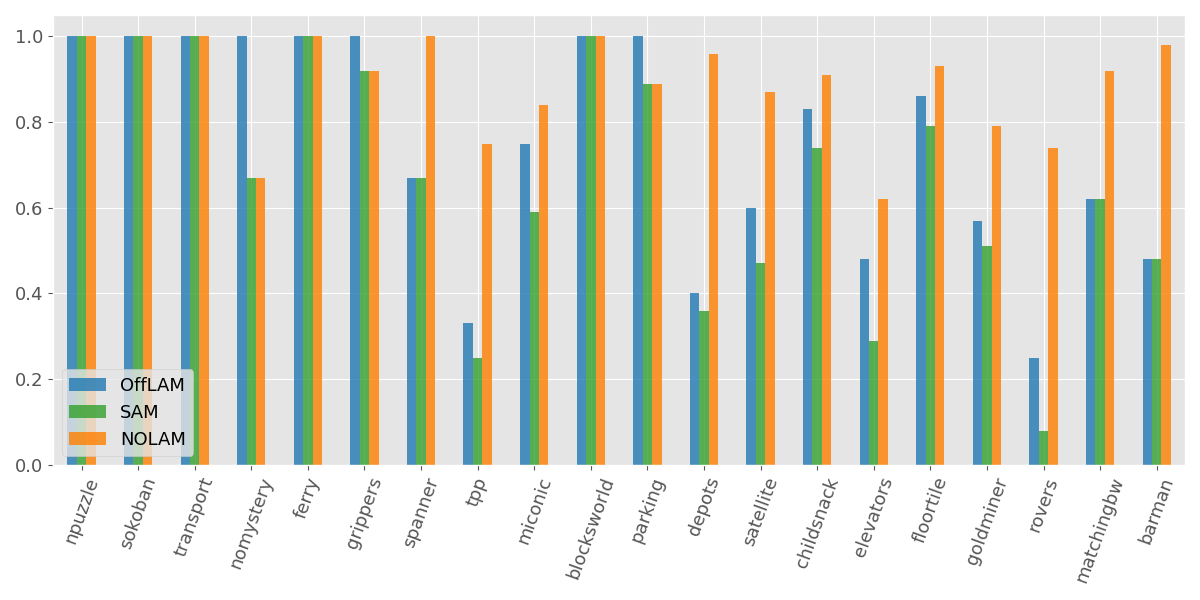
\includegraphics[width=\textwidth]{figures/2_traces/app_recall.png}
    \caption{Applicability recall}
  \end{subfigure}

  \vspace{1em}

  \begin{subfigure}[b]{0.45\textwidth}
    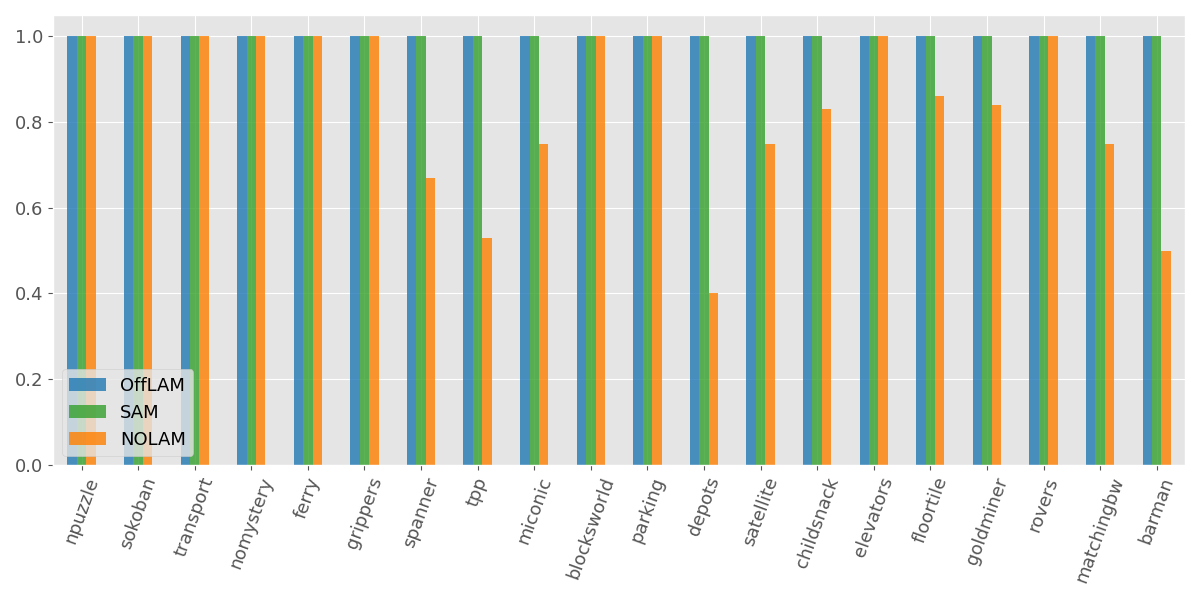
\includegraphics[width=\textwidth]{figures/2_traces/predeffs_precision.png}
    \caption{Predicted effects precision}
  \end{subfigure}
  \hfill
  \begin{subfigure}[b]{0.45\textwidth}
    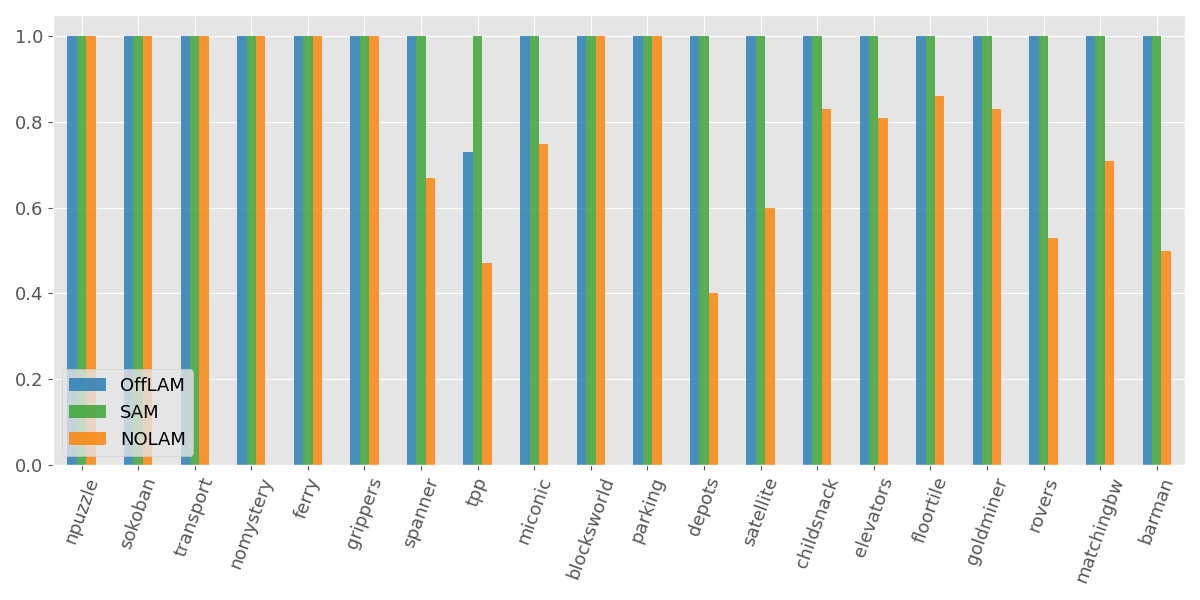
\includegraphics[width=\textwidth]{figures/2_traces/predeffs_recall.png}
    \caption{Predicted effects recall}
  \end{subfigure}

  \vspace{1em}

  \begin{subfigure}[b]{0.45\textwidth}
    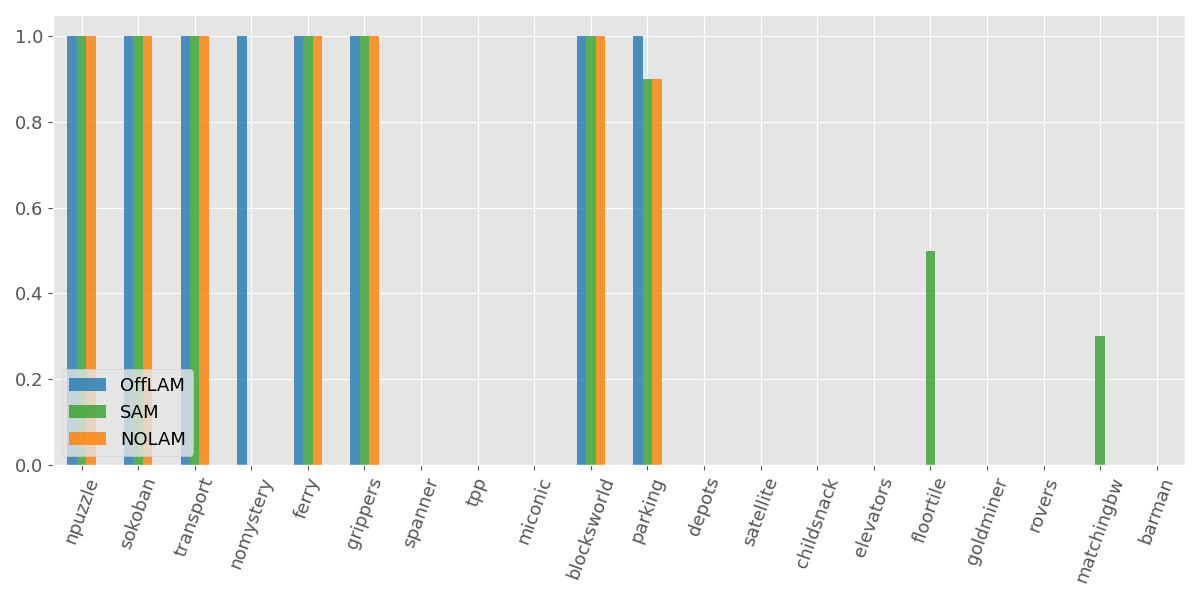
\includegraphics[width=\textwidth]{figures/2_traces/solving.png}
    \caption{Problem solving ratio}
  \end{subfigure}
  \hfill
  \begin{subfigure}[b]{0.45\textwidth}
    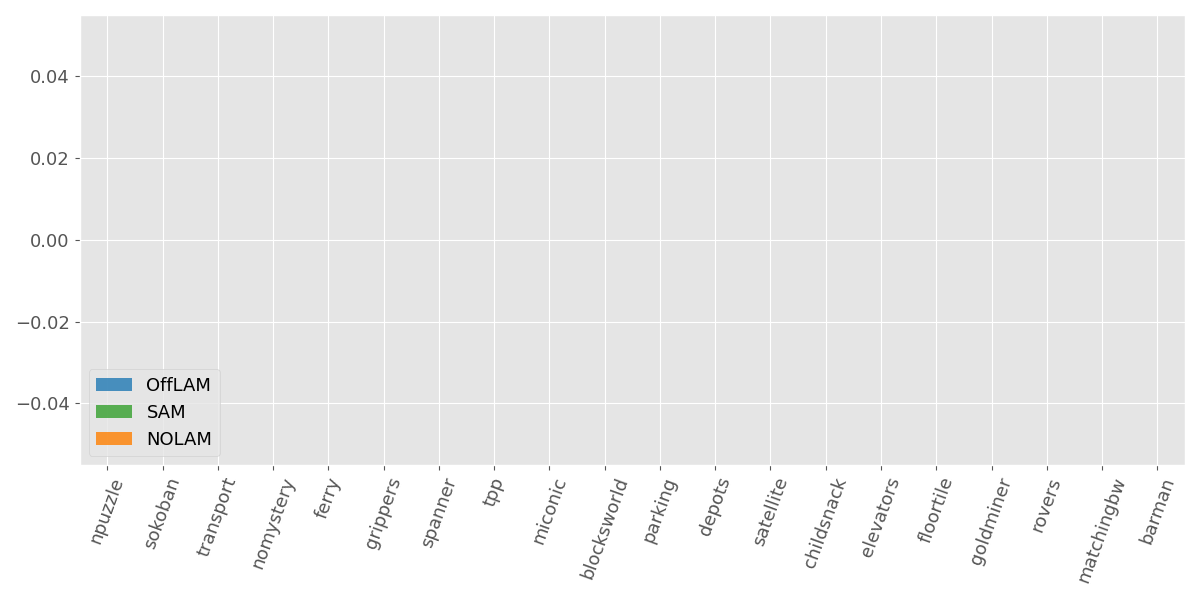
\includegraphics[width=\textwidth]{figures/2_traces/false_plans.png}
    \caption{False plans ratio}
  \end{subfigure}

  % \caption{Overall caption for the 6 images.}
  \caption{Evaluation metrics when learning from a training set $\hat{T}_{train}$ with $2$ traces for every domain.}
\end{figure} 